\section{Contrôle d'un agent via la simulation SE-STAR par renforcement profond}

Cette partie sera consacrée au fonctionnement du contrôle appliqué à SE-STAR. Dans le but de comprendre les choix entrepris, nous commencerons par expliquer comment fonctionne l'algorithme d'apprentissage par renforcement utilisé pour SE-STAR. Puis, nous expliquerons les faiblesses de cet algorithme (dans le contexte de SE-STAR). Enfin, nous introduirons un module de curiosité qui a pour but d'améliorer l'apprentissage et donc le contrôle de l'agent.


Nous considérons SE-STAR comme un environnement sans faire mention des problématiques liées à l'interface contrôleur / SE-STAR, ou des problématiques liés aux réseaux qui ont été développé dans la partie précédente. 

\subsection{Le choix d'un algorithme efficace pour le contrôle d'un agent dans SE-STAR.}

Il existe dans la littérature un panel très large d'algorithmes qui sont potentiellement puissants. Or, pour des questions de temps, nous n'avons pas été capable d'essayer tous les algorithmes. Nous avons donc dû faire un choix. 

Nous allons à travers cette partie, donner les principaux réseaux qui nous ont poussé à nous diriger vers un apprentissage par renforcement profond. 

Tout d'abord, les spécificités de SE-STAR impliquent le non-usage des algorihtmes \emph{model based} (basés sur un modèle, soit la connaissance de la fonction de transition). Or, il est évident que dans le cas de SE-STAR, cette fonction est inconnue. Nous pouvons même aller plus loin, la fonction de transition dans le cas d'états sous forme d'un tableau de pixels est bien souvent insoluble. Cela reviendrai à avoir la connaissance d'une fonction qui, sachant l'etat courant et l'action donne la probabilité d'être dans un nouvel état. Voici le cheminement pour déterminer le nombre de combinaisons possibles d'états pour une image de 82x82 pixels. Un pixel est composé de trois nombres de 0 à 255. Chaque pixel a la capacité de produire théoriquement $256^3 = 16\ 777\ 216\ \text{couleurs}$. Ainsi, il y a $82 * 82 * 256^3 = 112\ 810\ 000\ 384 \text{ combinaisons d'images différentes possibles}$. Nous comprenons vite l'impossibilité d'utiliser un algorithme basé sur la fonction de transition. Malgré le fait que pendant ce stage nous n'avons pas utilisé d'algorithmes purement \emph{model based}, nous pourrions toujours approximer cette fonction en utilisant une architecture de Deep Learning et en trouvant une fonction de perte adéquate.Cela est possible, mais ne sera pas testé durant ce stage car l'approche \emph{model based} est difficilement applicable dans le cas d'états sous forme de pixels (nous passons toujours par une phase de compression de l'état pour permettre ce genre d'algorithmes). Il y a peu d'algorithmes suivant ce principe qui ont montré de bon résultats sur des environnements difficiles.

\begin{itemize}
    \item Notre algorithme d'apprentissage par renforcement appartiendra à la famille des \textbf{algorithmes sans modèle (\emph{Model Free})}
\end{itemize}

Il existe beaucoup d'algorithmes dans la famille \emph{Model Free}. Nous souhaitons donc utiliser en premier lieu un algorithme qui est robuste et performant selon la littérature. De plus, nous aimerions un algorithme qui soit extensible. En effet, comme nous le verrons plus tard avec le module de curiosité, la plupart des environnements 3D sont  difficiles pour les algorithmes d'apprentissage par renforcement. 

Au vue de la littérature, il y a deux méthodes qui ressortent:
\begin{enumerate}
\item \bf{Deep Q Networks (DQN} \cite{mnih-dqn-2015})
\item Asynchronous advantage critic (\bf{A3C})\footnote{Nous utiliserons A3C ou DQN dans la suite de ce rapport} \cite{DBLP:journals/corr/MnihBMGLHSK16}
\end{enumerate}

Les principes sur lesquels reposent ces deux algorithmes ont été développé précédemment dans ce rapport. Bien que nous avons testé ces deux algorithmes sur SE-STAR, nous avons déjà commencé par comparer ces deux algorithmes sur des cas plus simples. Néanmois, il est à noter que sur les expérimentations, que nous avons effectué, ont été utilisées des versions améliorées du DQN de l'A3C (non indiquées dans ce rapport). En effet, ces méthodes ont trouvé un echo dans la communauté scientifique et ont été améliorées de nombreuses manières. Il serait trop long d'expliciter toutes les améliorations existantes pour ces algorithmes mais nous allons tout de même les citer et donner une référence pour les lecteurs les plus curieux.

% { -- GLOBAL CHANGE [[WARNING]]

\setlength{\arrayrulewidth}{.45mm}
\setlength{\tabcolsep}{12pt}
\renewcommand{\arraystretch}{2.}

\begin{center}
{\rowcolors{2}{white!80!gray!50}{gray!50!white!60}
\begin{tabular}{ |p{3.3cm}|p{11cm}|  }
\hline
\multicolumn{2}{|c|}{Algorithmes testés pendant le stage} \\
\hline
\multicolumn{2}{|c|}{\bf{Améliorations du Deep-Q-Network}} \\
\hline 
\textbf{Double-Q-Learning} (DDQN \cite{DDQN}) & Résout un problème intrinsèque du Deep Q Network qui est l'introduction d'un biais au niveau de l'estimation de la fonction d'état action.\\\hline


\textbf{Dueling-Q-Learning} \: (D-DQN\cite{DUEL}) & Au lieu d'approximer la fonction d'état action ($\rightarrow$ DQN), nous préférons approximer \emph{la fonction d'avantage} qui se défini comme la différence de la fonction d'état et de la fonction d'état action. Cela a de nombreuses qualités car la fonction avantage permet de déterminer si une action mène à un gain positif par rapport à la moyenne des gains espérée ce qui est plus utile que simplement la fonction d'état action dans le cadre du contrôle (la fonction avantage donne une information plus fine et intéressante que la fonction d'état action )  \\\hline

\textbf{Prioritized Replay}\cite{REPLAY} & Pour décoreller l'entraînement dans le cadre de l'apprentissage  en utilisant le DQN, nous sommes obligé de nous servir d'une mémoire pour stocker des transitions et pouvoir ensuite échantillonner celles-ci. La méthode de \emph{favorisation de la mémoire} consiste à échantillonner les transitions qui ont mené à la plus forte erreur (cf fonction de perte), ce qui correspond à des cas particulièrement intéressants dans le cadre de l'apprentissage.  \\\hline

\multicolumn{2}{|c|}{\bf{Améliorations de l'A3C}} \\
\hline 

\textbf{GAE}\footnote{Generalized Advantage Estimation tiré du papier: High-Dimensional Continuous Control Using Generalized Advantage Estimation }\cite{GAE} & La méthode GAE (voir note de bas de page pour avoir la référence) est une méthode qui n'est pas directement affiliée à l'A3C mais qui a été utilisée dans celle-ci et est devenu quasiment standard. L'idée est d'utiliser un estimateur de la fonction d'avantage qui est biaisé mais qui possède une variance plus faible. Il a été montré empiriquement que son utilisation améliore grandement l'apprentissage. \\\hline
\textbf{UNREAL}& A3C-GAE avec en plus des objectifs auxiliaires pour améliorer la stabilité du réseau et pousser l'agent à explorer son environnement.
\\\hline
\end{tabular}
}
\end{center}


Comparons empiriquement les méthodes dérivées du DQN et de l'A3C.

\subsection{Comparaison entre les méthodes issues de la famille du DQN et de l'A3C}

\subsubsection{Les algorithmes issus de la famille du Deep Q Learning}

% TODO -------------------------

Les résultats sont issus d'expérimentations sur l'environnement de contrôle cartpole, où le but est de maintenir une barre sur un ensemble mobile le plus longtemps possible. L'ensembles des actions est composé de LEFT pour aller à gauche et RIGHT  pour aller à droite. L'agent reçoit une récompense de +1 à chaque pas de temps. L'environnement est réussi lorsque que l'agent a 200 points (nombre de points maximum).

\begin{center}
    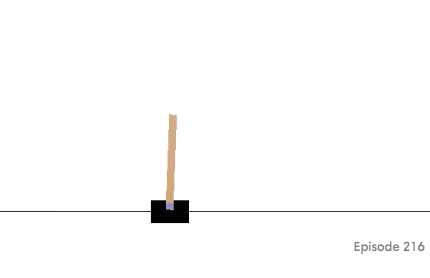
\includegraphics[scale=.5]{./assets/DeepLearning/cartpole.png}
\end{center}

\begin{figure}[H]

\begin{minipage}{.5\linewidth}
\centering
\subfloat[]{\label{main:a}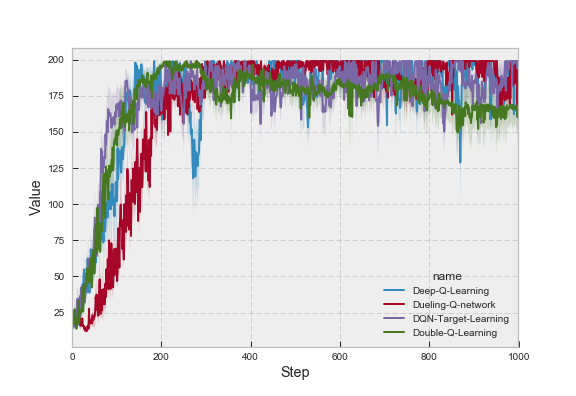
\includegraphics[width=1\linewidth]{./assets/DQNResult/4}}
\end{minipage}%
\begin{minipage}{.5\linewidth}
\centering
\subfloat[]{\label{main:b}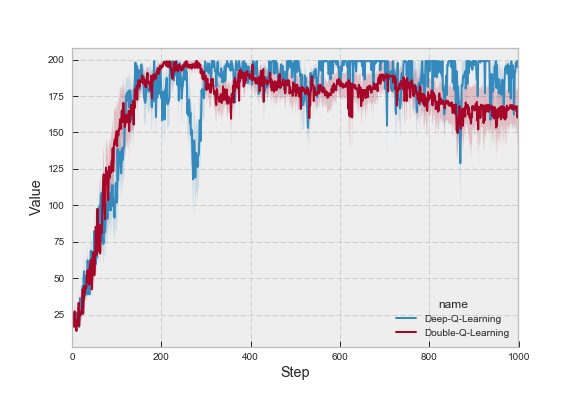
\includegraphics[width=1\linewidth]{./assets/DQNResult/2}}
\end{minipage}\par\medskip

\begin{minipage}{.5\linewidth}
\centering
\subfloat[]{\label{main:a}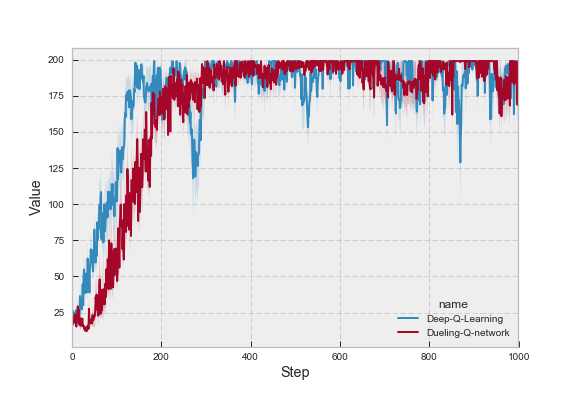
\includegraphics[width=1\linewidth]{./assets/DQNResult/3}}
\end{minipage}%
\begin{minipage}{.5\linewidth}
\centering
\subfloat[]{\label{main:b}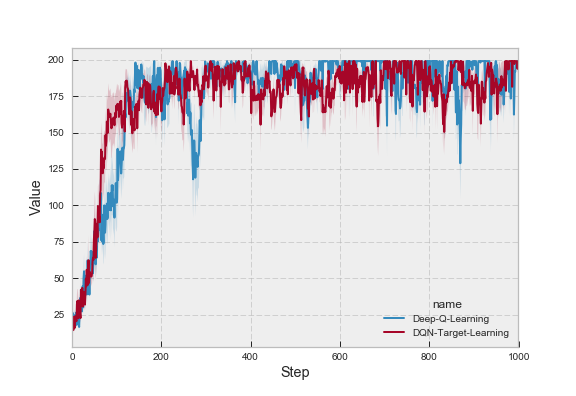
\includegraphics[width=1\linewidth]{./assets/DQNResult/1}}
\end{minipage}\par\medskip
\caption{Résultats du Deep Q learning sur CartPole}
\label{fig:main}
\end{figure}

A travers ces premiers résultats, nous pouvons comparer les différents algorithmes issues de la famille du Q Learning.

Nous pouvons remarquer que, quelque soit l'algorithme issu de la fammile du Q Learning, l'apprentissage est dans l'ensemble stable. En effet, Nous ne voyons pas, pour la majorité des algorithmes testés,  de chutes de performance durant l'apprentissage. Cependant, il y a de faibles différences concernant la dynamique d'apprentissage. L'algorithme le plus simple (\emph{le Deep-Q-Learning} a la dynamique la plus rapide pour arriver de façon quasiment stable à 200 points avec le Deep-Target-Learning\footnote{une version du DQN visant à stabiliser l'apprentissage}}. Ceci s'explique car les dérivés du DQN stabilisent l'entraînement au prix d'un apprentissage plus long. 
Il est à noter que tous les autres algorihtmes issus du Q learning ont été testés dans la version avec \emph{Target}. Nous pouvons ainsi voir que, globalement, le DQN est un peu moins stable que les autres algorithmes (présence de pics avec un score faible). Enfin, nous pouvons constater que \emph{le dueling-Q-network} et le DQN avec target sont les plus stables et donc les plus adéquats.

Ce constat est corrélé avec d'autres expérimentations faites qui ne sont pas présentent dans ce rapport.


\subsubsection{Les algorithmes issus de la famille de l'A3C}

\begin{figure}[h]

\begin{minipage}{.5\linewidth}
\centering
\subfloat[]{\label{main:a}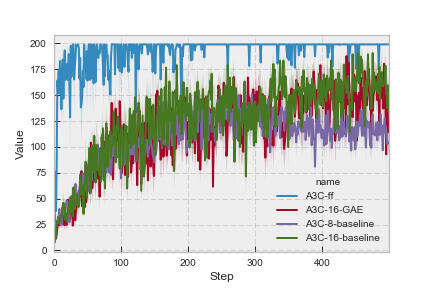
\includegraphics[width=1\linewidth]{./assets/A3CResult/11}}
\end{minipage}%
\begin{minipage}{.5\linewidth}
\centering
\subfloat[]{\label{main:b}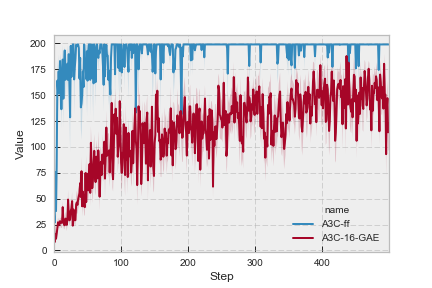
\includegraphics[width=1\linewidth]{./assets/A3CResult/22}}
\end{minipage}\par\medskip

\begin{minipage}{.5\linewidth}
\centering
\subfloat[]{\label{main:a}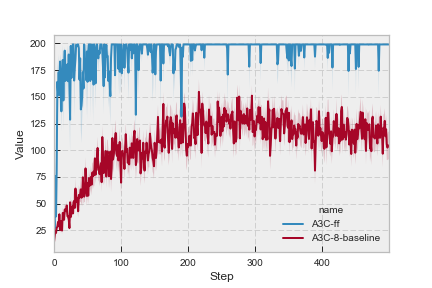
\includegraphics[width=1\linewidth]{./assets/A3CResult/33}}
\end{minipage}%
\begin{minipage}{.5\linewidth}
\centering
\subfloat[]{\label{main:b}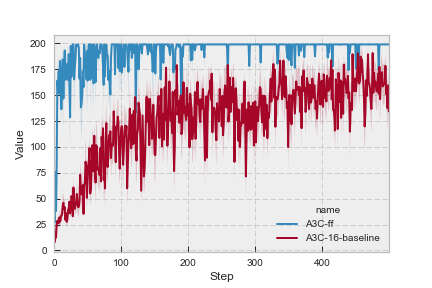
\includegraphics[width=1\linewidth]{./assets/A3CResult/44}}
\end{minipage}\par\medskip

\caption{Résultats de l'A3C sur CartPole}
\label{fig:main}
\end{figure}

Nous avons réalisé les mêmes expérimentations avec des algorithmes issus de la famille de l'A3C. Nous avons testé en particulier deux variantes de l'A3C.
\begin{itemize}
    \item A3C-FF \\
        Pour A3C Feedforward, cela fait référence au type de réseau de neurones utilisé en sortie du réseau de convolution. En particulier, le réseau de neurones correspond au modèle ldense précédement décrit.
    \item A3C-LSTM \\
        LSTM correspond à un réseau de neurones récurrent qui a la particularité par rapport au réseau dense de prendre en compte les états précédents. Ce type de réseau est pertinant dans le cas où nous avons seulement une image partielle de l'environnement.
\end{itemize}
De plus, nous avons comparé ces types d'algorithmes avec un nombre différent de processus. Rappelons que l'A3C est un algorithme asynchrone se basant sur de multiples agents (dans la littérature entre 4 et 32 processus sont habituellement utilisés) 
Nous remarquons que l'A3C est quasiment deux fois plus rapide que le DQN (et ses variantes) pour arriver au score maximum de 200 points dans sa verison Feedforward (FF). Cela s'explique car un réseau récurrent est bien plus long à entrainer. Pour des applications complexes nous préférerons la version LSTM de l'A3C. Ainsi, dans le cadre de SE-STAR, nous utiliserons la version LSTM.

Le nombre de processus est aussi déterminant dans la dynamique d'apprentissage. En regardant la figure c qui compare la version FF avec 16 processus (en bleu) et la version avec 8 processus, nous nous rendons compte qu'un nombre élevé de processus est bénéfique pour l'entraînement.

Cartpole est un environnement relativement simple à résoudre. L'environnement est éloigné de notre cas d'usage qui sera SE-STAR. Nous avons donc testé les différents algorithmes sur des environnements plus complexes. 
Ci dessous, les résultats pour différents environnements 2D dans lesquels l'état est un tableau de pixels (82*82). Ces environnements sont plus complexes que Cartpole pour au moins trois raisons. 
La première est qu'il y a un nombre élevé d'actions (douze en moyenne), la deuxième est que l'état possède une haute dimensionnalité. Enfin, les récompenses sont données seulement à la fin d'un épisode ou  plus rarement que dans Cartpole. Cela ralenti l'entraînement assez fortement et posera de nombreux problèmes.  


\begin{figure}[H]

\begin{minipage}{.5\linewidth}
\centering
\subfloat[]{\label{AAA}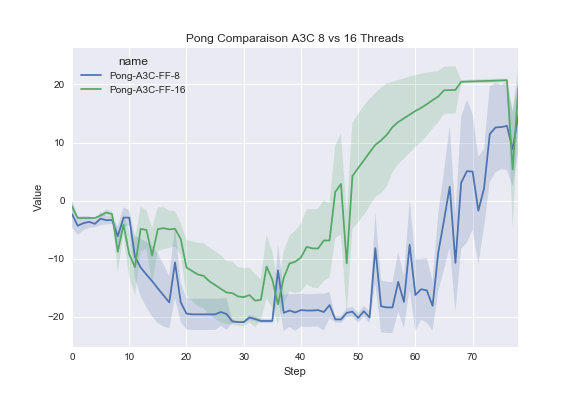
\includegraphics[width=1\linewidth]{./assets/ATARI_RESULT/pong.png}}
\end{minipage}%
\begin{minipage}{.5\linewidth}
\centering
\subfloat[]{\label{BBB}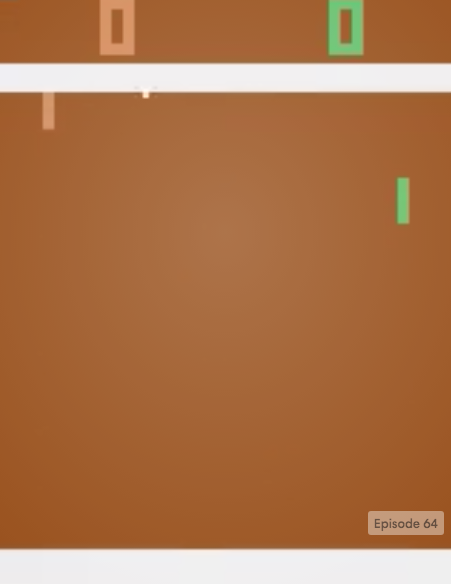
\includegraphics[width=.6\linewidth]{./assets/ATARI_RESULT/pong1.png}}
\end{minipage}\par\medskip

\begin{minipage}{.5\linewidth}
\centering
\subfloat[]{\label{main:Seaquest}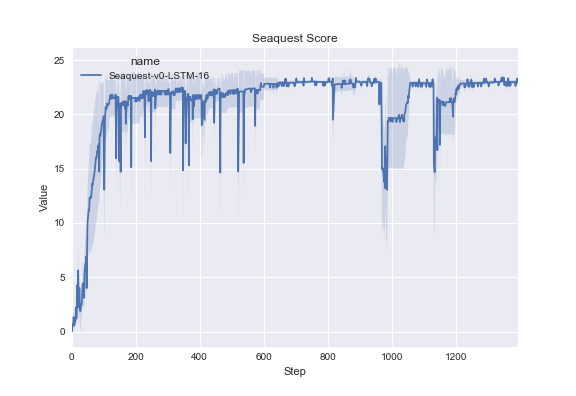
\includegraphics[width=1\linewidth]{./assets/ATARI_RESULT/Seaquest.png}}
\end{minipage}%
\begin{minipage}{.5\linewidth}
\centering
\subfloat[]{\label{main:b}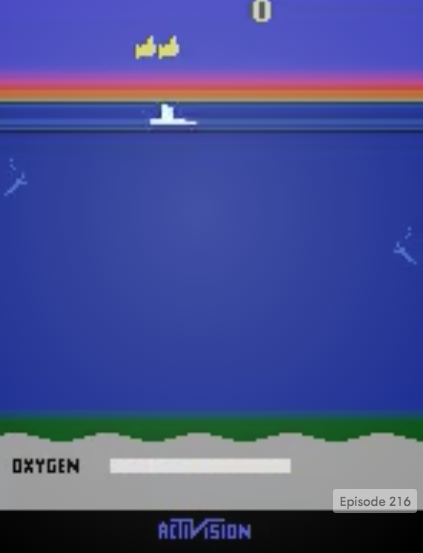
\includegraphics[width=.6\linewidth]{./assets/ATARI_RESULT/Sequest1.png}}
\end{minipage}\par\medskip


\begin{minipage}{.5\linewidth}
\centering
\subfloat[]{\label{main:a}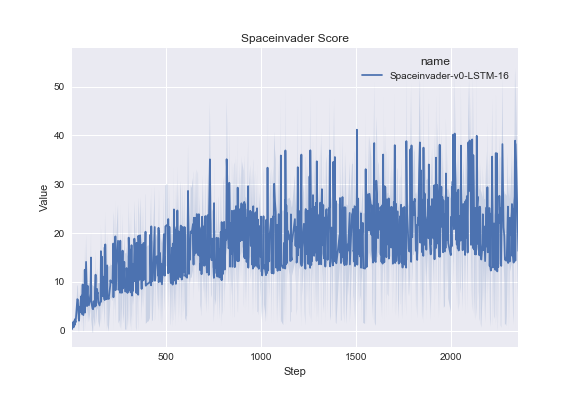
\includegraphics[width=1\linewidth]{./assets/ATARI_RESULT/Spaceinvader.png}}
\end{minipage}%
\begin{minipage}{.5\linewidth}
\centering
\subfloat[]{\label{main:b}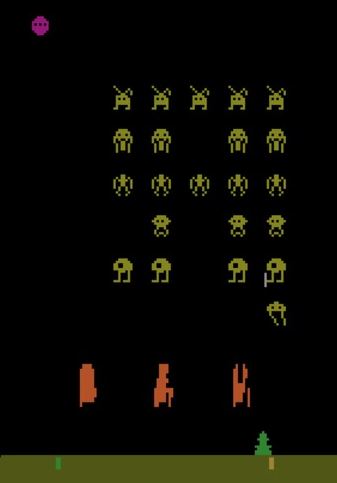
\includegraphics[width=.6\linewidth]{./assets/ATARI_RESULT/Spaceinvader1.png}}
\end{minipage}\par\medskip


\caption{Résultats de l'A3C sur des environnements ATARI}
\label{fig:main}
\end{figure}

Nous avons utilisé l'A3C-LSTM-GAE pour l'apprentissage car il a montré de meilleurs résultats d'après nos tests. Nous n'avons pas utilisé un algorithme issu de la famille du Q-Learning car un des défault de cette famille est la lenteur pour converger vers une bonne politique. Nous avons déjà mentionner qu'intrinsèquement le Deep-Q-Learning avait des problèmes de stabilité, or les stratégies pour le stabiliser ont aussi pour effet d'entraver la dynamique d'apprentissage de celui-ci. Dans la suite de ce rapport, nous privilégierons donc les méthodes se basant sur la famille de l'A3C.

\subsection{Spécification des différents environnements créés par SE-STAR}

Dans cette partie, nous introduirons les environnements qui ont été utilisés avec notre architecture de contrôle. Nous avons créé plusieurs environnements et plusieurs représentations (images 2D vue de haut, vue FPS\footnote{Vue classique des jeux vidéo d'action, où l'on voit seulement ce que l'agent voit}). Nous montrerons qu' à l'heure actuelle, certains environnements sont difficiles à utiliser avec de l'apprentissage par renforcement pour des raisons que nous verrons ultérieurement.

\subsubsection{Environnement labyrinthique simple créé par SE-STAR}

L'objectif de ce stage fut de contrôler un agent à travers un environnement labyrinthique dans le but de trouver la sortie de celui-ci. Notre premier environnement fut extrêmment simple. 

Ci-dessous, une image de l'environnement créé et de la representation associée à celui-ci.


\begin{figure}[h!]
\centering
\begin{minipage}{.5\textwidth}
  \centering
  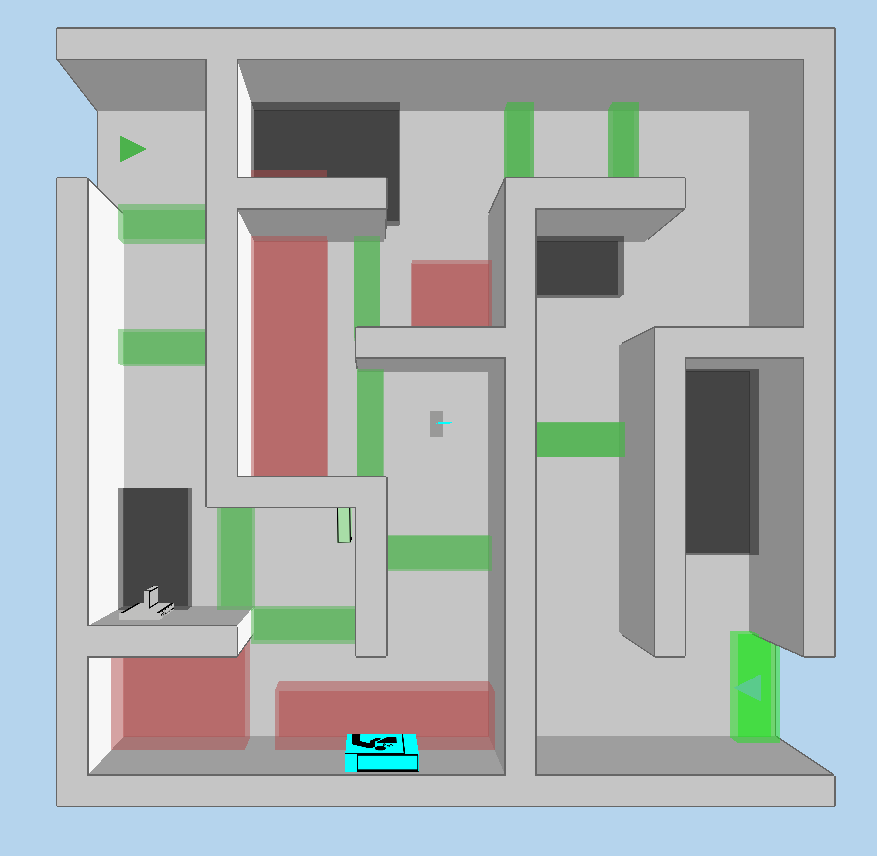
\includegraphics[width=.5\linewidth]{./assets/SESTAR/env_sestar_agent.png}
  \caption{Environnement A en 3D}
  \label{fig:test1}
\end{minipage}%
\begin{minipage}{.5\textwidth}
  \centering
  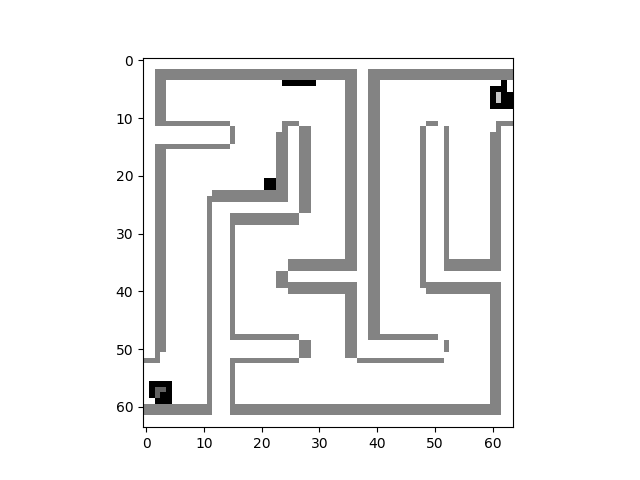
\includegraphics[width=.65\linewidth]{./assets/SESTAR/vue_agent_1.png}
  \caption{\small{Environnement A par l'agent}}
  \label{fig:test2}
\end{minipage}
\end{figure}

\todo[inline]{Transformer en tiré ou tableau}
Nous pouvons voir en rouge les coins où l'agent va recevoir une pénalité de -0.1, et en vert foncés les coins où l'agent va recevoir une récompense de +0.1. Le coin en vert clair représente l'arrivé souhaitée (avec une récompense de +1). Les lieux en noir sont des lieux où l'agent est très fortement pénalisé (par une pénalité de -1) et une interruption de l'environnement (équivalent à un game over\footnote{partie perdue dans un jeux video}). Quand l'agent passe dans une zone où il reçoit une récompense, toute la zone disparait pour éviter des stratégies où l'agent tournerait en rond dans une zone à récompenses. 

Ci-dessous un tableau récapitulatif des spécifications de l'environnement:


\rowcolors{2}{blue!10}{blue!25}
\begin{center}
    \begin{tabular}{|c|c|}
    \Xhline{2\arrayrulewidth}
    \multicolumn{2}{|c|}{Spécifications} \\
    \Xhline{2\arrayrulewidth}
    Gestion des actions & De 4 à 9 actions (modulables) \footnotemark\\
    Durée des actions & Quatres pas de temps \\
    Format de l'état&2D\\
    Taille de l'image & 42 * 42\\
    Prise en compte de l'orientation& Oui\footnotemark\\
    \Xhline{2\arrayrulewidth}
\end{tabular}
\end{center}
\footnotetext{On utilisera les actions suivantes: HAUT, BAS, DROITE, GAUCHE, DIAGONALES (4 actions), et NO-OP (ne rien faire)}

\footnotetext{Les actions ont un effet différent en fonction de l'orientation}

Nous avons noté un apprentissage très difficile avec ce type d'environnement. Cela est principalement dû à des problèmes réseaux qui ont ralenti et complexifié l'entraînement. Néanmoins, nous avons noté que l'état donné à l'agent était difficilement exploitable. Un problème avec la représentation qu'on a adopté (en 2D) est l'absence de vision du placement des récompenses. Or, comme nous l'avons déjà noté, pour réussir un apprentissage, l'agent doit être capable de récupérer des informations pertinantes de l'état. Cela n'est pas possible avec la représentation actuelle.

Nous avons donc utilisé le même environnement avec une représentation. Ci-dessous, la véritable image sortie du simulateur et l'image donnée à l'agent pour l'apprentissage.

\begin{figure}[h!]
    \begin{center}
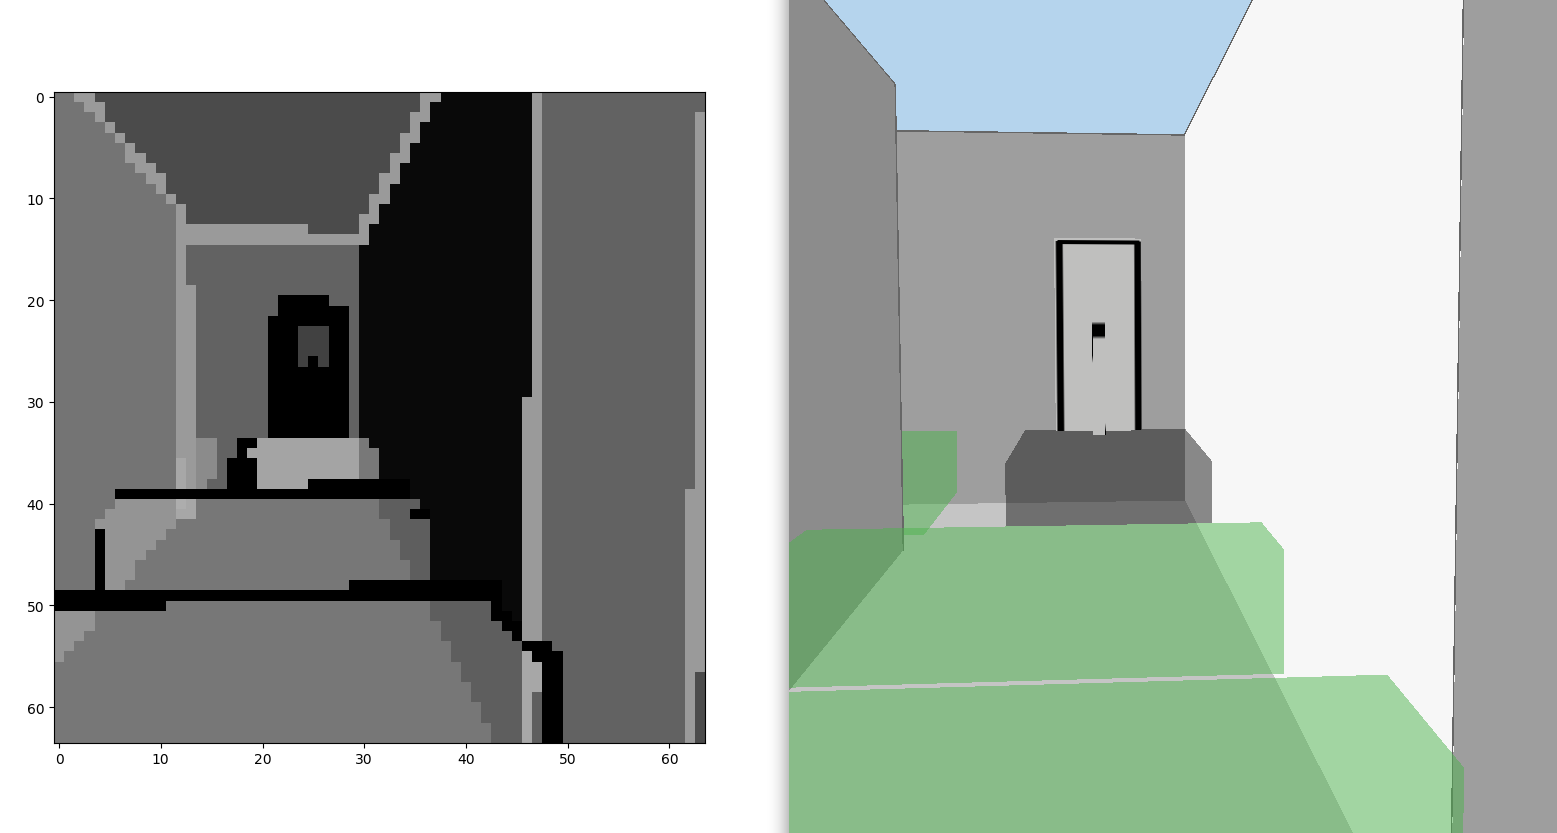
\includegraphics[scale=.15]{./assets/SESTAR/se2.png}
\caption{Représentation 3D de l'environnement}
\end{center}
\end{figure}

Comme le montre les figures au dessus, la vue est partielle et correspond à ce que voit l'agent. Les zones de récompenses sont maintenant visibles mais le résultat n'est pas satisfaisant. En effet, avec la nouvelle représentation qui est une vue 2D partielle est particulièrement difficile pour notre agent. Les environnements 3D avec une vue 2D donnés à un agent sont complexes pour des agents entraintés via A3C (ou DQN). Cela s'explique car ce genre d'algorithmes utilise une architecture qui cherche des éléments saillants dans l'environnement pour pouvoir approximer la Q fonction et trouver la politique optimale. Or dans notre environnement il y a peu d'élements possiblement interessants pour approximer la Q fonction. De plus, la Q fonction (ou fonction d'état-action) donne une estimation de la valeur d'une action suivant une politque. Le problème est que nous utilisons des actions qui dépendent fortement de l'orientation de l'agent. Si l'agent choisit d'avancer, selon l'orientation de celui-ci, l'action AVANCER aura un sens radicalement différent du point de vuede l'agent. Cela implique que l'approximation recherchée est quasiment impossible.


Pour régler un maximum de problèmes, nous avons créé  un environnement similaire qui possède plus d'éléments caractéristiques  pour aider l'agent. Nous avons supprimé la dépendance par rapport à l'orientation de l'agent. 


\begin{figure}[h!]
    \begin{center}
        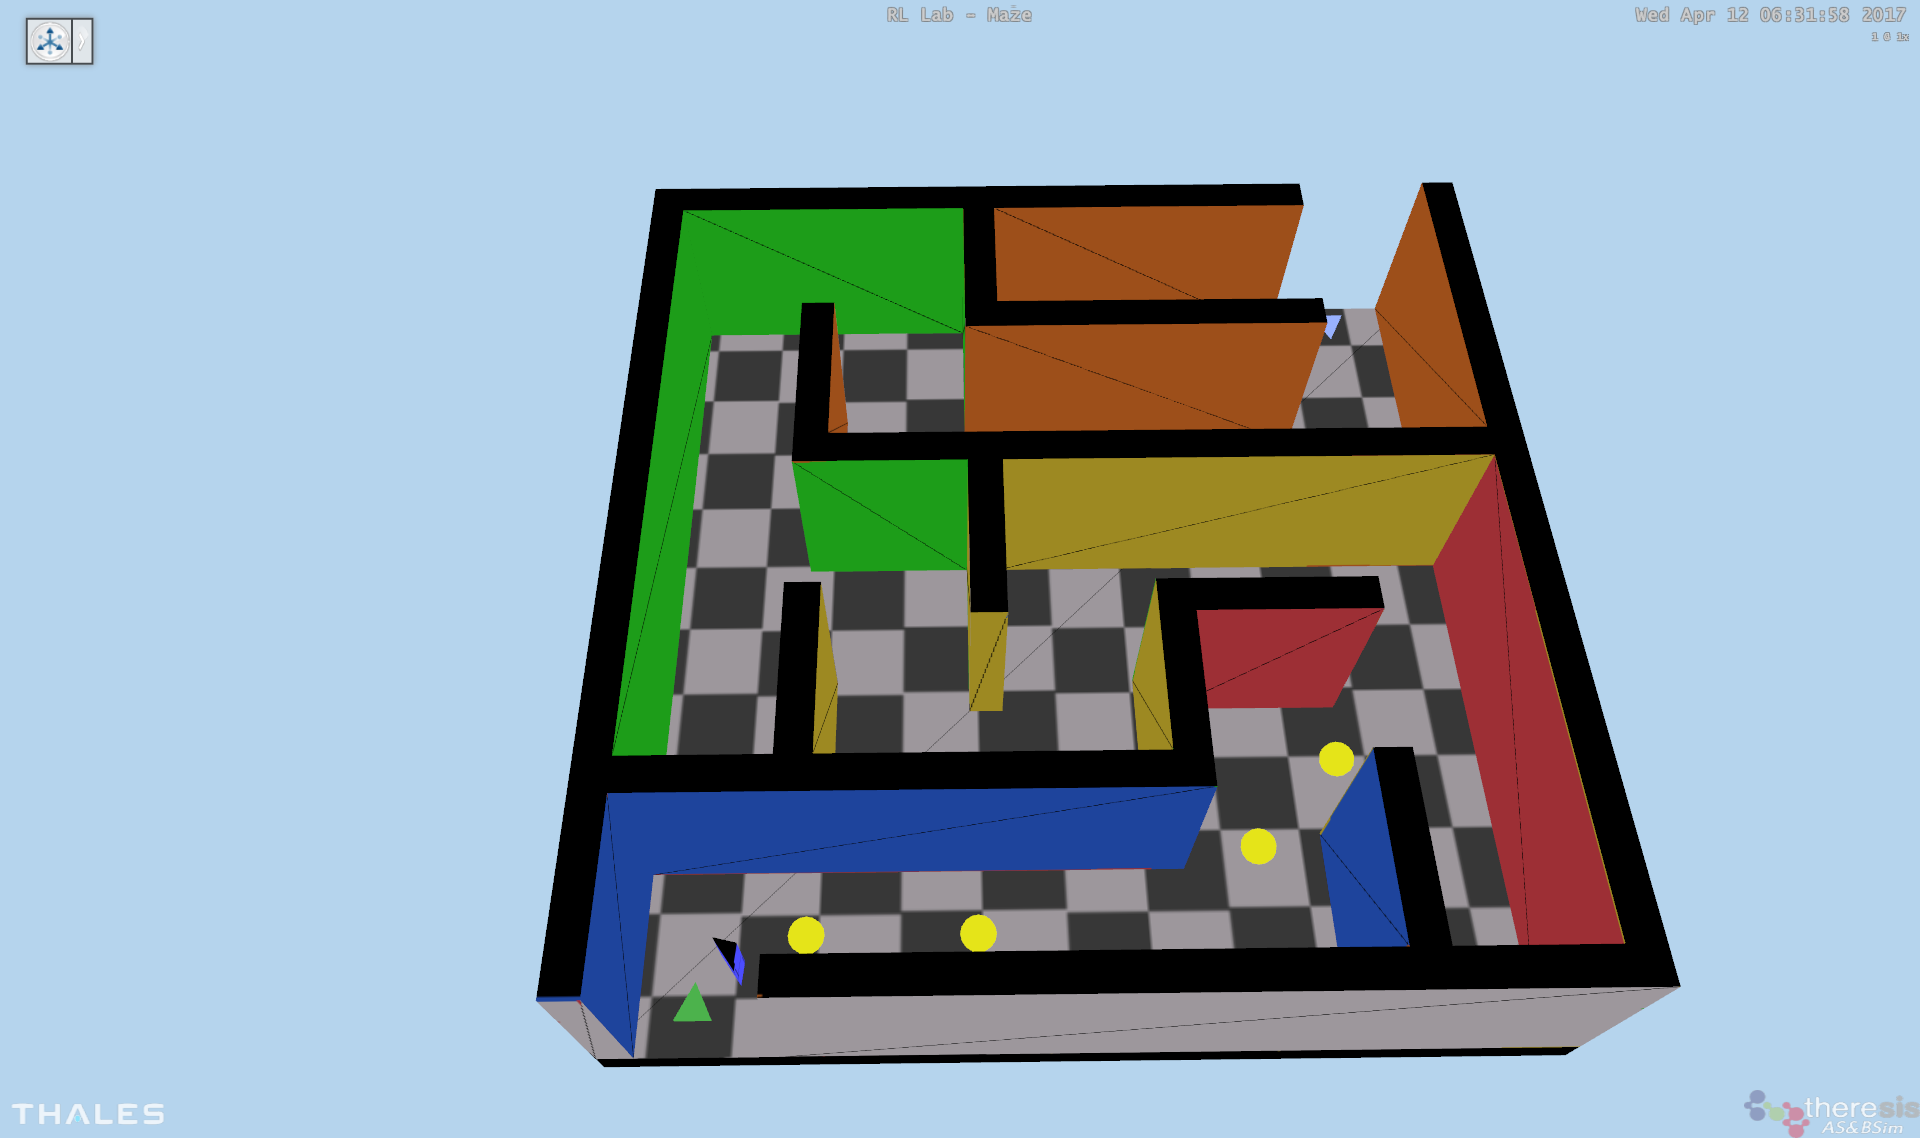
\includegraphics[scale=.15]{./assets/SESTAR/env_sestar_color.png}
\caption{Représentation 3D de l'environnement B}
\end{center}
\end{figure}

Comme nous le voyons, l'environnement est plus coloré pour permettre à l'agent un apprentissage plus aisé. La spécification reste globalement la même sauf pour la dépendance par rapport à l'orientation. 

\rowcolors{2}{red!10}{red!25}
\begin{center}
    \begin{tabular}{|c|c|}
    \Xhline{2\arrayrulewidth}
    \multicolumn{2}{|c|}{Spécifications} \\
    \Xhline{2\arrayrulewidth}
    Gestion des actions &  4 actions (modulables) \footnotemark\\
    Durée des actions & Quatres pas de temps (modulables) \\
    Format de l'état&3D\\
    Taille de l'image & 42 * 42\\
    Prise en compte de l'orientation& Non \\
    \Xhline{2\arrayrulewidth}
\end{tabular}
\end{center}

Avec cet environnement, nous avons une bonne base d'expérimentation. Malheureusement, nous n'avons pas pu expérimenter autant de temps que nous l'aurions voulu. Nous avons pu démontrer avec cet environnement qu'il était possible de faire intéragir des algorithmes d'apprentissages par renforcement avec un logiciel de simulation qui n'était pas adapté à cela. Compte tenu des résultats que nous avons eu, nous avons décidé d'intégrer des mécanismes de curiosité dans notre contrôle pour permettre à l'agent d'explorer l'envrionnement de façon beaucoup plus efficace. 

Le manque d'exploration a été une difficulté majeure pour l'agent. Des stratégies utilisant des motivations auxiliaires ont été mises au point pour répondre à ce problème. Nous explorerons cette idée dans la partie suivante.


